%% V1.0
%% 2021/28/11
%% Developed by Alex Gimenez Romero on top of Techset-developed templates.

\documentclass[openacc]{rsproca_new}

\usepackage{amsmath}
\usepackage{url}
\usepackage{multicol}

\addbibresource{refs.bib}
\providecommand{\aiuse}[1]{{\vskip5.5pt\noindent \textcolor{jobcolor}{\fontsize{9}{11}\selectfont Use of Artificial Intelligence (AI) and AI-assisted technologies.}\fontsize{8}{11}\selectfont\enskip #1}}


\jname{rsif}
\Journal{J R Soc Interface\ }

\begin{document}

\title{Fine-scale locomotor actuation leaves detectable pressure signatures in fish wakes}

\author{Bastien Lagneaux$^{1}$, Corentin Porcon$^{1}$, Michael Mabelle$^{2}$, Paul Lagneaux$^{3}$, Thomas Omarini$^{1}$, Boai Sun$^{1}$, Nadia Maria Hamilton$^{4}$, Florence Razan$^{1}$, James Herbert-Read$^{4}$, Gurvan Jodin$^{1}$}

\address{$^{1}$Univ Rennes, ENS Rennes, CNRS IETR -- UMR 6164, Rennes, France\\
$^{2}$AMIAD, France\\
$^{3}$Université Bourgogne Europe, Institut Agro, INRAE, UMR PAM, Dijon, France\\
$^{4}$Department of Zoology, Cambridge University, Cambridge, United Kingdom}

\subject{biomechanics, biological fluid dynamics, sensory ecology}

\keywords{fish wake, lateral line, digital twin, vortex persistence, computational fluid dynamics, wake sensing}

\corres{Bastien Lagneaux\\
\email{bastien.lagneaux@ens-rennes.fr}}

\begin{abstract}
Fish can sense hydrodynamic information left by other swimmers, but how such information contributes to behavioural decisions, including predator–prey interactions or conspecific following, remains unclear. We combined sparse wall-pressure measurements with two-dimensional numerical wake models driven by observed trajectories of striped eel catfish, \textit{Plotosus lineatus}. A deforming fish-shaped digital twin and a cylinder surrogate followed the same measured centre-of-mass paths, and interpretable classifiers compared simulated pressure segments with experimental measurements. Measured segments were more consistently associated with the deforming fish model than with the cylinder, especially when streamwise body-surface deformation was retained. At $95\%$ retained pressure-mode variance, the x-deformation model classified $30.3\%$ of measured pressure segments as fish-like and $4.4\%$ as cylinder-like with a $0.99$ confidence threshold. Vortex-level interpretation indicated that displacement, spatial position, path geometry and persistence were more informative than raw vortex intensity alone. These results do not directly demonstrate behavioural use of wake cues. Rather, they suggest that fine-scale body deformation contributes substantially to hydrodynamic information in fish wakes, with implications for lateral-line sensing, individuality in wake signature and hydrodynamic communication.
\end{abstract}

\begin{fmtext}
\end{fmtext}

\maketitle
\section{Introduction}
Swimming animals generate hydrodynamic wakes, spatio-temporal flow structures, that encode information about body size, trajectory and motion history \cite{weihs1975}. Fish can sense such flow signatures through sensory organs such as the lateral line system, which responds to pressure gradients and velocity fluctuations associated with nearby vortical structures \cite{drucker2000, videler2002, coombs1988}. Wake sensing has been shown to contribute to behaviours including schooling and have been associated with energetic benefits in collective motion \cite{liao2003}, but the way these cues are structured in the wake of a freely swimming fish remains difficult to study directly.

Experimental access to the full wake is usually limited. Flow measurements around live animals can perturb the animal or cover only part of the domain. A common strategy in fluid mechanics is therefore to replace the swimming animal with a simplified body, such as a cylinder or other canonical bluff geometry. Such surrogates are valuable because they isolate elementary wake mechanisms and make simulation or experimental control tractable. However, their biological validity depends on the question being asked. A following fish is unlikely to encounter only the centre-of-mass trajectory of a leader. It may instead encounter a wake shaped by detailed body form, deformation and local surface motion. The biological question is therefore not whether a cylinder can generate a wake, but which swimming parameters (path, form, deformation) are responsible for preserving pressure and vortex signatures.

Here, a fish-shaped deforming digital twin and a cylinder surrogate driven by the same experimentally observed paths were compared. Because the full experimental wake was not measured directly, wall-mounted pressure signals were used as sparse, non-invasive measurements. A classifier trained only on simulated fish and cylinder pressure segments was then used as a comparative consistency metric for measured pressure segments. In this manuscript, ``fish-like'' means more consistent with the deforming fish digital twin in the learned pressure-signal space. It is not interpreted as direct evidence of behavioural cue use, communication or individual recognition.

\section{Materials and methods}

\subsection{Experimental data, wake models and sample accounting}

The data used in this work originated from infrared video recordings of striped eel catfish, \textit{Plotosus lineatus}, swimming in a water tank equipped with wall-mounted pressure sensors. The recordings were acquired at 100 frames s$^{-1}$ with an image resolution of 2000 $\times$ 1200 pixels. Fish body contours and sensor locations were visible in the same view, allowing fish motion to be related to the pressure signals measured at the wall.

\begin{figure}[b]
    \centering{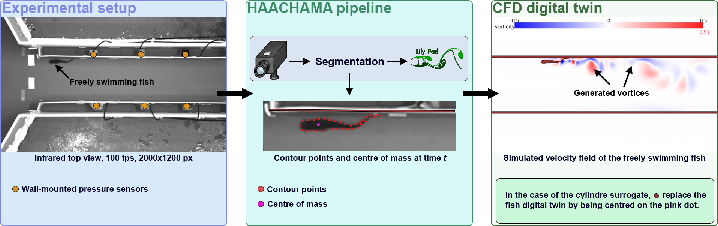
\includegraphics[width=1\linewidth]{figures/haachama.pdf}}
    \caption{Overview of the HAACHAMA pipeline used to generate a deforming fish-shaped digital twin and a cylinder surrogate. Infrared video recordings provided the fish trajectory and body contour, and wall-mounted pressure sensors provided the only direct experimental access to the wake. The fish-shaped digital twin and the cylinder surrogate were driven by the same centre-of-mass trajectory.}
    \label{fig:haachama}
\end{figure}

The raw dataset contained 40 videos segmented into 493 discrete samples where the fish was visible. Fish body contours were extracted from each video sequence using the HAACHAMA pipeline \cite{lagneaux2024,lagneaux2025}, summarised in Figure \ref{fig:haachama}. Each frame was represented by a closed contour, and each sequence described both displacement and deformation of the fish body through time. These contours were used to generate a deforming, fish-shaped computational digital twin in LilyPad \cite{maertens2015}. The same contours provided the fish centre-of-mass trajectory, which drove a cylindrical surrogate with diameter set by fish body width. The digital twin and cylinder therefore shared the same observed path but differed in body shape and deformability. 403 samples were retained after applying the HAACHAMA pipeline, corresponding to 81.7\% of the segmented samples. These samples are made out of 367 of the 375 samples which were successfully processed by the pipeline without manual intervention, 17 of the 20 samples which needed a heavy-cropping before being processed, 6 out of the 11 poorly segmented samples (meaning the contour was visibly off for some frames) and 13 of the 16 samples in which the fish was segmented as a cylinder for a few frames during the sample. The complete breakdown of sample validity and retention is given in table \ref{tab:sample_breakdown}.

Four model variants were compared. The raw digital twin used the original contour sequence. The size-constrained variant imposed a constant contour length to reduce frame-to-frame segmentation variability. The x-deformation variant allowed both streamwise and transverse body-surface motion to contribute to the moving-boundary forcing. The full variant combined the size constraint and streamwise-deformation addition. For the cylinder surrogate, the size constraint had no effect because the geometry was already fixed. This variant was thus identical to the raw variant, as well as the streamwise-deformation to the full variant.

\begin{table}[t]
\centering
\caption{Validity breakdown of the samples of the dataset}
\label{tab:sample_breakdown}
\begin{tabular}{p{0.5\linewidth}r r r}
\hline
Category & Samples & Valid & Invalid\\
\hline
Successfully processed & 375 & 367 & 8\\
Heavy temporal cropping required & 20 & 17 & 3\\
Poor segmentation & 11 & 6 & 5\\
No detection in some frames & 26 & 0 & 26\\
Fish not fully submerged / 3D interaction & 18 & 0 & 18\\
Fish did not pass in front of sensors & 26 & 0 & 26\\
Circular segmentation error, tail touching nose & 16 & 13 & 3\\
External interference, flake in water & 1 & 0 & 1\\
\hline
\textbf{Total} & \textbf{493} & \textbf{403} & \textbf{90}\\
\hline
\end{tabular}
\end{table}

\subsection{Using sparse pressure measurements to evaluate wake realism}

Because several retained pressure segments can originate from the same recording, and therefore be generated by the same individual fish, potential video-level dependence among retained measured-pressure segments was assessed separately using a measured-pressure Singular Value Decomposition (SVD) space and same-video versus different-video distance comparisons. Details are provided in the supplementary material.

Direct experimental access to the full wake was not available, so model consistency was evaluated using pressure signals measured at wall sensors. Simulated pressure signals were extracted at sensor locations during the passage of tracked vortices. Vortices were identified from simulated velocity fields using the Q-criterion \cite{hunt1988,kolar2007},
\begin{equation}
Q=\frac{1}{2}\left(\lVert \Omega \rVert^2-\lVert S \rVert^2\right),
\end{equation}
where $\Omega$ and $S$ are the antisymmetric (rotation) and symmetric (strain) components of the velocity-gradient tensor. Positive values of $Q$ indicate regions where rotational motion dominates over deformation and are used to detect coherent vortices. Vortex trajectories were retained only when they passed through a sensor-sensitive region and remained sufficiently far from the generating body to reduce contamination by immediate body passage.
    
Pressure values at the sensor locations were extracted at each time step for which at least one valid vortex was present. Segments were labelled according to the model that generated them: fish-shaped digital twin or cylinder. Segments were then mean-centred, amplitude-normalised and resampled to a common length. SVD was used to construct pressure-mode bases retaining 75\%, 95\% or 99\% of simulated variance \cite{klema1980}. A deliberately simple linear classifier was trained to distinguish fish-generated from cylinder-generated simulated pressure segments. Its purpose was to provide a task-specific comparative metric, not a new machine-learning architecture \cite{hadsell2006,pacchiardi2021,tkachev2021}.

Measured pressure segments were processed in the same way and projected into the same reduced feature spaces. Because the classifier learned only the difference between two simulated model classes, a measured segment classified as fish-like was interpreted as more consistent with the fish-shaped model than with the cylinder surrogate in that feature space. Low-confidence outputs were assigned to an undetermined class. Confidence thresholds from 0.50 to 0.99 were analysed.

The key points of the method described in this subsection are illustrated in Figure \ref{fig:classifier}. The details regarding the training of this first-stage classifier, including the training procedure, hyperparameters and performance metrics, are provided in the supplementary material, as well as more details about the data base. The files needed to reproduce this study are available at \cite{lagneaux2026}.

\begin{figure}[t]
    \centering{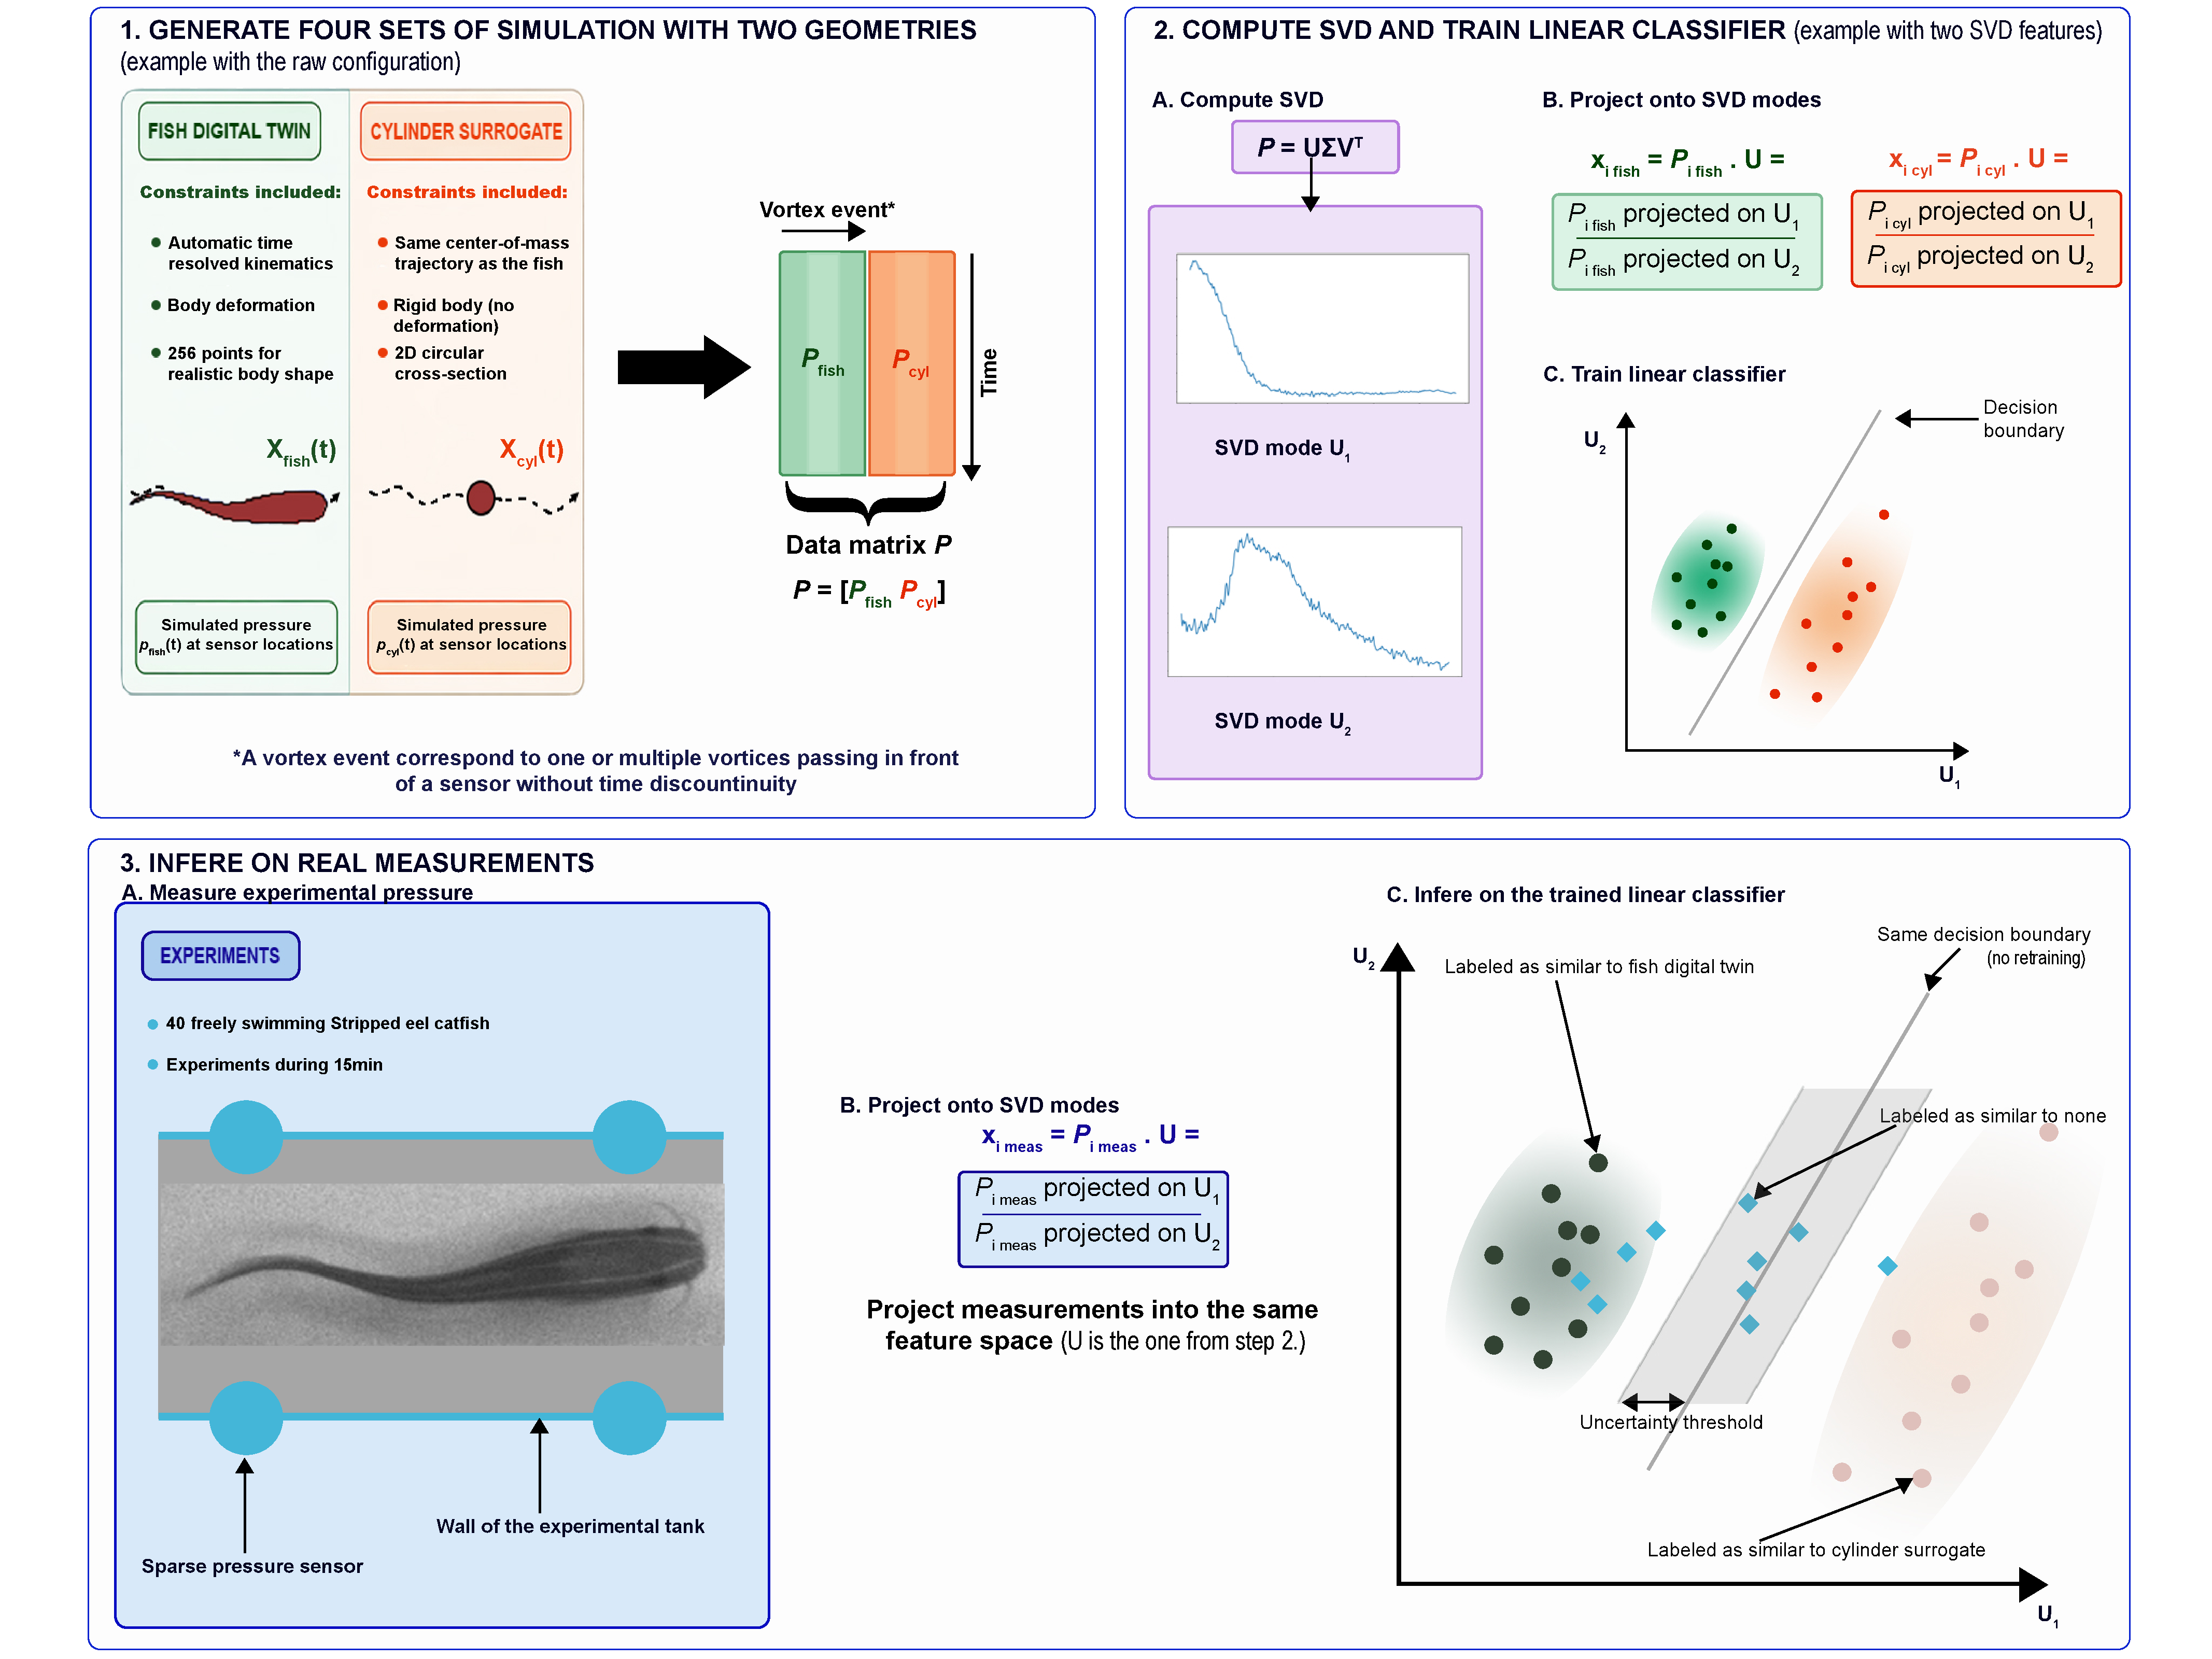
\includegraphics[width=1\linewidth]{figures/classifier.pdf}}
    \caption{Schematic representation of the methodology. (1) Simulation stage: fish-shaped digital twin and cylinder surrogates are generated under different model variants (raw, size-constrained, x-deformation and full). Pressure signals are extracted from vortex tracking and assembled into a data matrix. (2) Dimensionality reduction and classification training: SVD is applied to construct a reduced basis capturing most of the dataset variance. Pressure signals are projected onto this basis to form feature vectors, used to train a linear classifier into distinguishing fish-like and cylinder-like simulations, hence defining a learned similarity metric. (3) Inference: experimental pressure signals are projected onto the same feature space and evaluated with this metric.}
    \label{fig:classifier}
\end{figure}

\subsection{Interpreting which vortex features carry fish-specific information}

To relate pressure-based labels back to wake structure, labels from the pressure classifier were propagated to the vortices associated with each signal segment. A second linear classifier was trained using interpretable vortex descriptors, including vortex duration, displacement, path length, distance to the body, distance to the sensor, speed, radius, area, Q-criterion magnitude and mean core position. SHAP (SHapley Additive exPlanations) values were used to estimate which descriptors contributed most to classification as fish-like or cylinder-like \cite{lundberg2017}. This step was used to link biological labels and physical content of the classifier decision, in other words to interpret how fish-specific information is linked with vortex representation, but not to infer behaviour directly.

\section{Results}

\subsection{Classifier performance and uncertainty}
The video-level dependence analysis showed limited clustering of measured-pressure segments by recording identity. In a measured-pressure SVD space retaining 99.1\% of variance, the variance-weighted one-way intraclass correlation coefficient ICC(1) was 0.058, indicating that video identity accounted for approximately 6\% of the retained measured-pressure variance. Same-video samples were also only about 6\% closer than different-video samples in standardised SVD space. A video-wise split was therefore not necessary when assigning pressure segments to analysis subsets. Details regarding the computation of these metrics are available in the supplementary materials.

The first-stage classifier showed that fish-shaped and cylinder simulations were separable but overlapping. Test accuracies are available in the supplementary material for each variant model and each level of retained variance. These moderate accuracies support comparative use of the classifier but do not justify treating classification as direct wake reconstruction.

\subsection{Measured pressure signals were more consistent with the fish-shaped model}

Across most model variants and confidence thresholds, measured pressure segments were classified more often as fish-like than as cylinder-like. This indicated that the deforming fish-shaped digital twin preserved pressure features consistent with the measured wake that were not captured by the cylinder surrogate following the same centre-of-mass trajectory. For experimental biology applications, this means matching the observed path of a fish is not sufficient, and though the fish-shaped model should not be considered a perfect reconstruction of the experimental wake, this is evidence that body shape and deformation contributed information that was consistent with the experimental data. 

The strongest separation occurred when streamwise deformation was included. For the x-deformation model with the 95\% retained-variance basis, 132 of 436 measured segments were classified as fish-like at the 0.99 confidence threshold (30.3\%, 95\% Wilson binomial CI 26.2--34.7\% \cite{wilson1927}), whereas 19 of 436 were classified as cylinder-like (4.4\%, 95\% Wilson binomial CI 2.8--6.7\%). The remaining segments were undetermined at that threshold. The difference between fish-like and cylinder-like fractions remained approximately constant across confidence thresholds from 0.50 to 0.99 (Figure \ref{fig:result95SVD}).

\begin{figure}[t]
    \centering{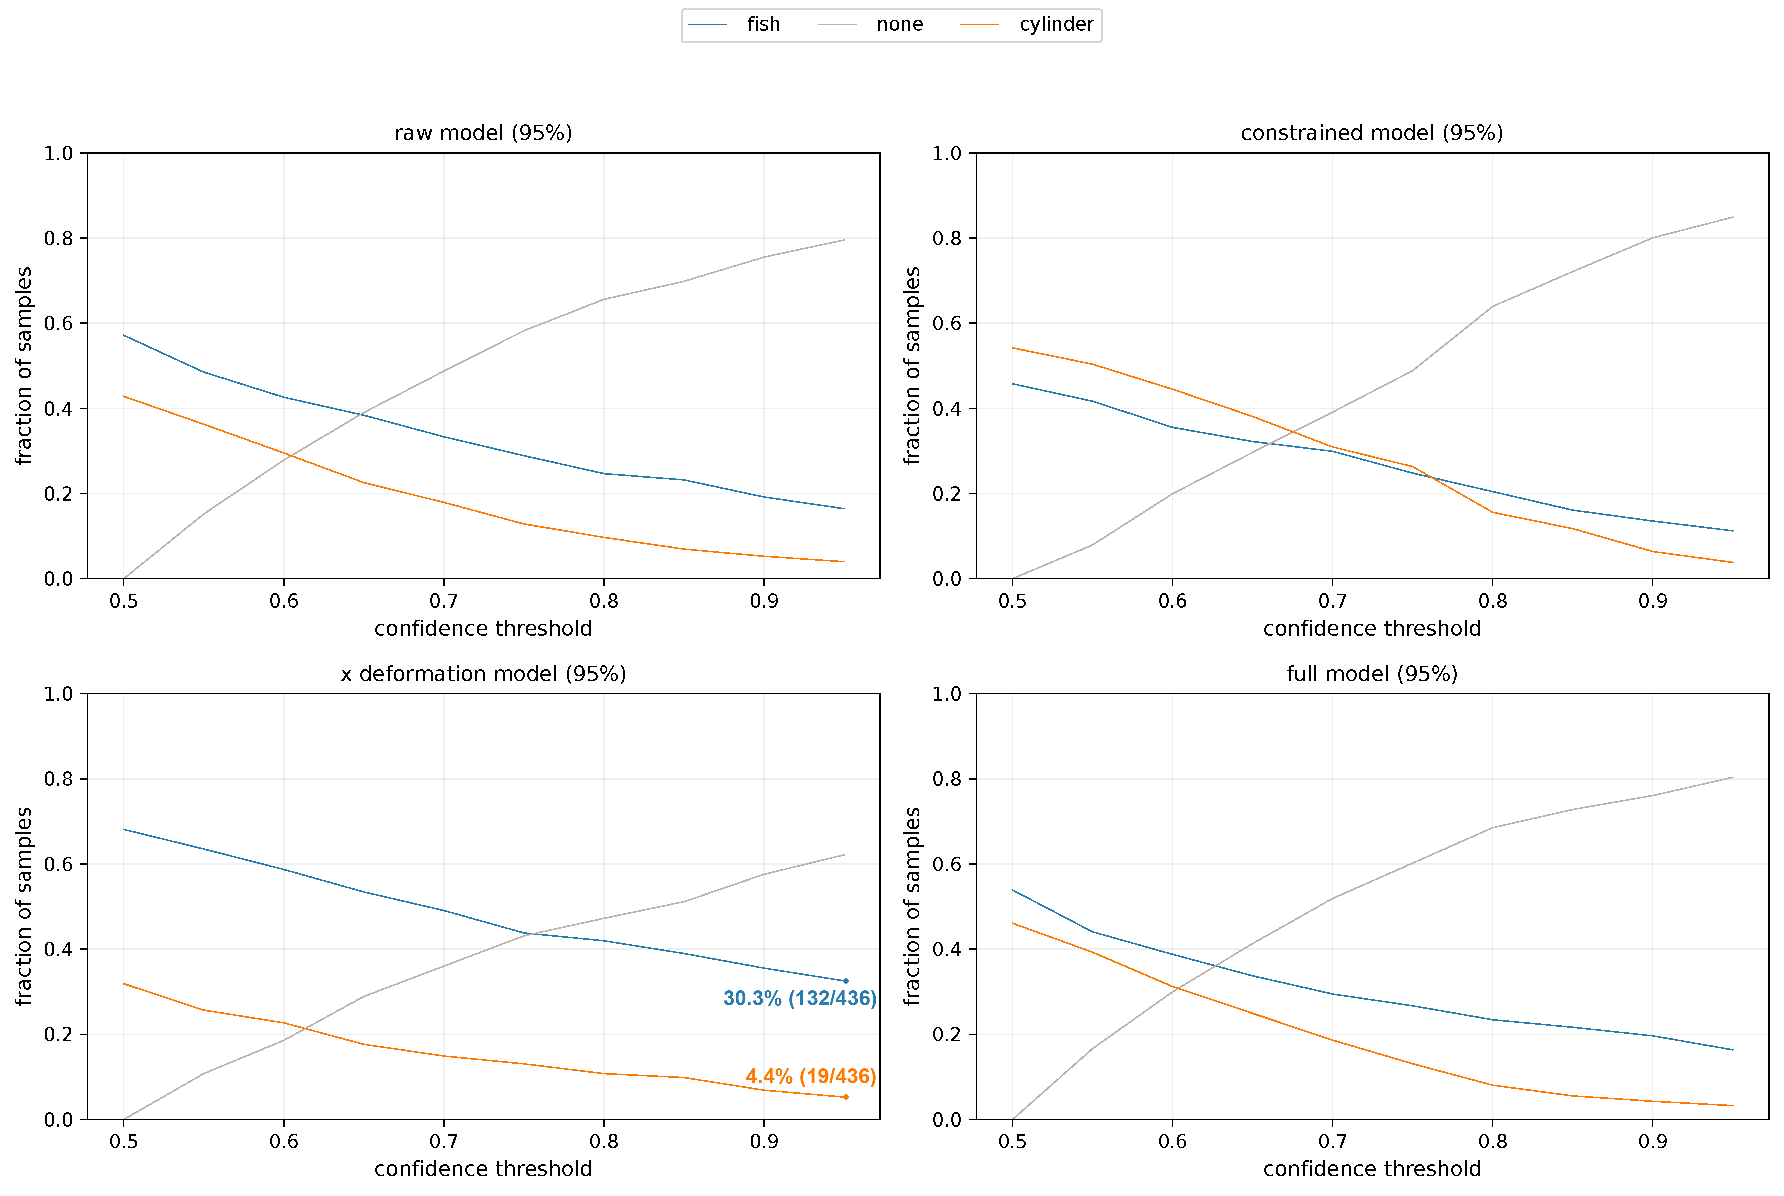
\includegraphics[width=1\linewidth]{figures/real_pressure_threshold_curves_95.pdf}}
    \caption{Fractions of measured pressure-signal segments classified as fish-like, cylinder-like or undetermined when 95\% of variance was retained. Across most configurations, measured signals were more frequently associated with the fish-shaped model than with the cylinder surrogate.}
    \label{fig:result95SVD}
\end{figure}

The 75\% and 99\% retained-variance bases showed the same pattern (for figures, see supplementary material). This consistency suggests that the effect was not an artefact of a single dimensionality-reduction choice. It also indicates that the discriminative pressure information was not confined only to the highest-energy modes.

\subsection{Parameters for wake realism: streamwise deformation, size constraint}
\subsubsection{Streamwise deformation contributed to wake realism}

Allowing streamwise as well as transverse body deformation to force the fluid produced the most consistent improvement in agreement with measured pressure signals. The input contour sequence was unchanged and only the moving-boundary forcing was modified. This points to a physical interpretation: longitudinal redistribution of the body surface, local stretching and compression, and other in-plane components of body motion contribute measurably to pressure signatures that reach the sensors.

This is important because fish locomotion is often described primarily in terms of lateral body undulations and centre-of-mass \cite{li2021,sfakiotakis1999}. The present results suggest that, for wake cues analysis, streamwise components of the body-surface motion should not be treated as negligible implementation details. They can influence the hydrodynamic signature left behind the swimmer and may therefore affect the information available to downstream receivers.

\subsubsection{Size constraint did not improve agreement with measured signals}

The size-constrained model did not improve agreement of the fish-shaped model with measured signals. Instead, it made the fish-shaped and the cylinder-shaped models harder to distinguish, and measured signal classification less stable across the confidence threshold variation. The full model, which included the size constraint as well as streamwise deformation, showed similar patterns and also failed to improve agreement over the streamwise deformation model alone. A plausible interpretation is that apparent contour-size variability in the single-camera reconstruction was not purely segmentation noise. Because the fish was a three-dimensional swimmer viewed in two dimensions, projected contour changes may partly encode out-of-plane motion, body roll or posture-dependent shape changes. Removing this variability may therefore remove real projected information as well as segmentation artefacts. This strengthens the interpretation that fine-scale body deformation's impact on the wake is not negligible.

\subsection{Vortex descriptors emphasized persistence and geometry}

The vortex-feature analysis focused on the x-deformation model with 95\% retained variance and a 0.99 confidence threshold. SHAP analysis indicated that the most influential descriptors were vortex displacement (the length of the straight line between the initial and final positions of the vortex), mean distance to the generating body, mean core x-position, path length (the total distance travelled by the vortex) and duration. Fish-like classification was therefore associated primarily with where vortices travelled, how far they moved, how long they persisted and how their trajectories developed, rather than with vortex size or intensity alone. 

These results are illustrated in Figure \ref{fig:shap} relative to the analysed subset, where cylinder-like vortices (represented by positive values on the x-axis) tended to be shorter-lived, with shorter (blue points) duration values and smaller average positions. These same vortices were also more intense when generated but decaying more rapidly, as shown by the combination of the mean and maximum radius values and by the average speed, and more rectilinear, as demonstrated by the displacement and path length ratio. On the other hand, fish-like vortices (represented by negative values on the x-axis) were more persistent, weaker, hence slower to decay, and followed more curved and spatially distributed paths.

\begin{figure}[t]
    \centering{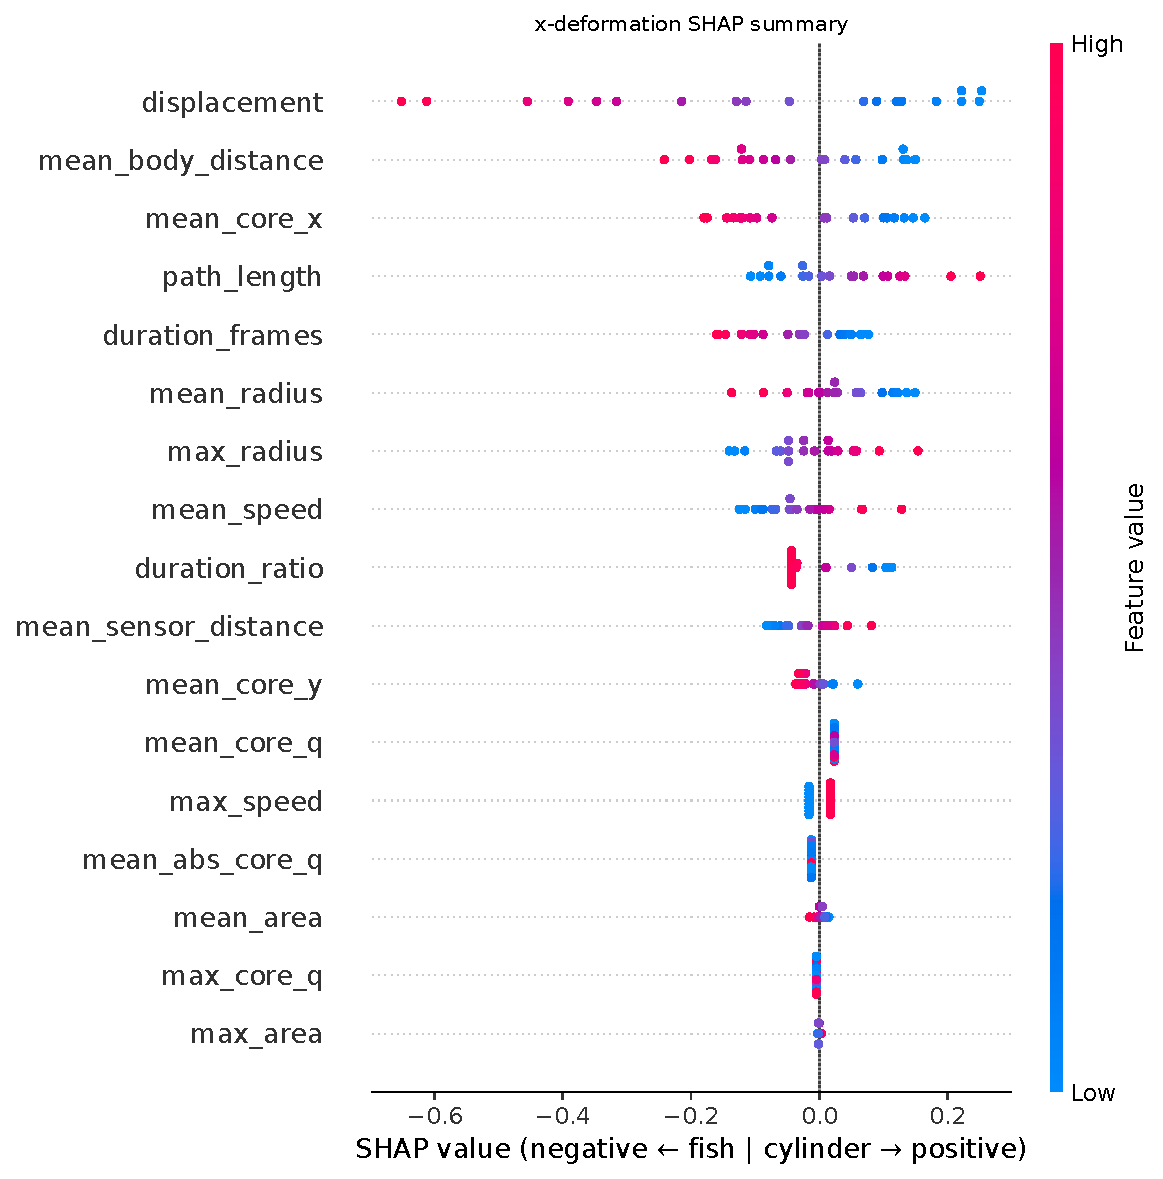
\includegraphics[width=1\linewidth]{figures/vortex_shap_boai_95_thr0.99.pdf}}
    \caption{SHAP summary plot for the second stage vortex-feature classifier. The most informative descriptors were related to vortex displacement, distance from the body, streamwise position, travelled path and duration, hinting that fish-specific information was expressed primarily through spatial organisation and persistence of vortical structures.}
    \label{fig:shap}
\end{figure}

The pattern found in these results could be the consequence of cylinder-like vortices being partly driven by near-body transient. When the minimum allowed distance between a vortex and the generating body was varied between 3 and 12 simulation grid mesh (x-axis in Figure \ref{fig:distance_filter}), fish-like classifications fraction increased for the four model variants when near-body structures were excluded more strongly . In the x-deformation subset, the baseline distance filter of 6 grid mesh gave 30.3\% fish-like and 4.4\% cylinder-like measured segments at the 0.99 threshold. Halving the minimum distance reduced the fish-like fraction to 24.8\% and increased the cylinder-like fraction to 10.6\%. Doubling the minimum distance increased the fish-like fraction to 37.9\%, while the cylinder-like fraction was 7.2\%. These trends support the interpretation that cylinder surrogate indeed reproduced some immediate short-lived near-body disturbances which might be associated with body passage, whereas persistent downstream structures were more consistent with the deforming fish model. This distinction is biologically relevant because a trailing fish is more likely to sample the wake after the leader has moved on, and therefore encounter vortical structures that have persisted and travelled downstream rather than instantaneous disturbances associated with body passage.

\begin{figure}[t]
    \centering{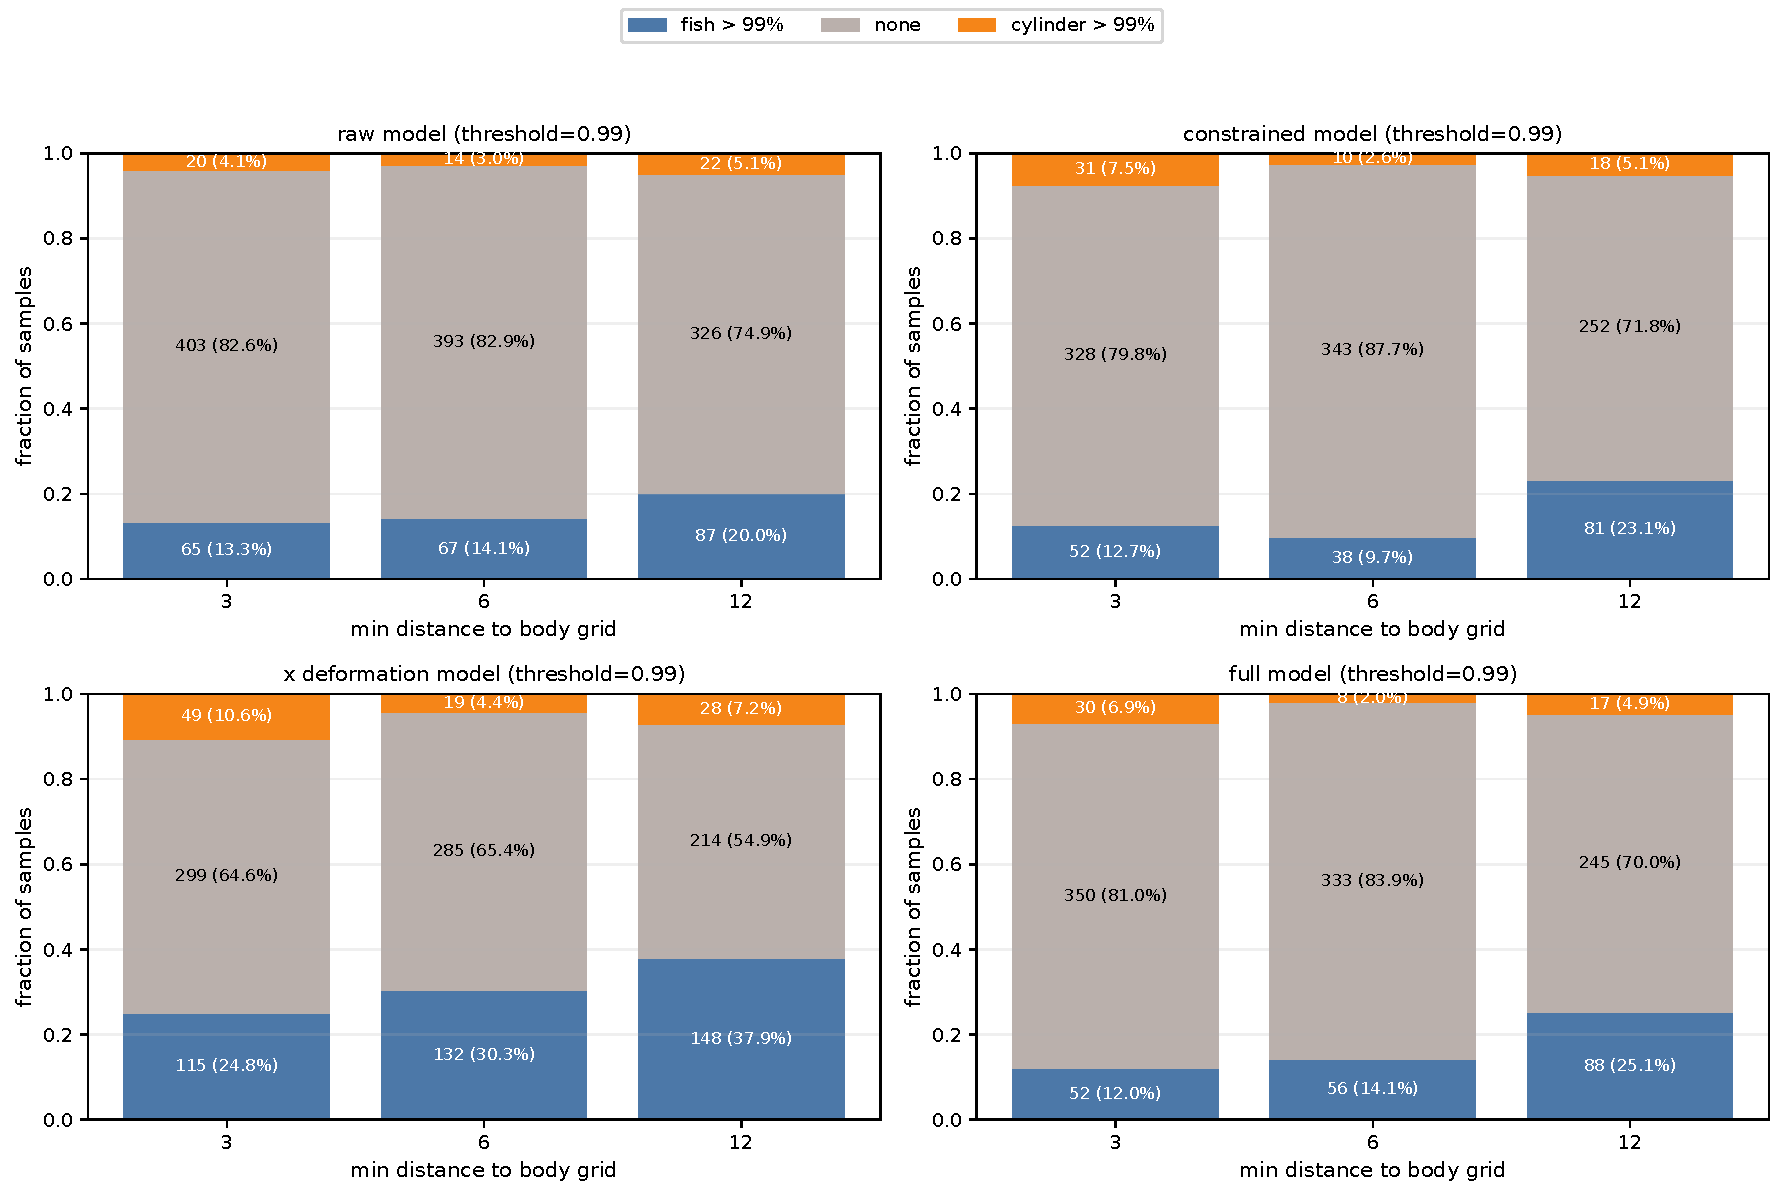
\includegraphics[width=1\linewidth]{figures/paper_ready_distribution_min_distance.pdf}}
    \caption{Effect of the minimum body-distance filter on measured signal classification at 99\% confidence. Increasing the exclusion of near-body vortices strengthened the association between measured pressure signals and fish-shaped digital twin.}
    \label{fig:distance_filter}
\end{figure}

\section{Discussion}
\subsection{Fine-scale body deformation implementation for biological realism of wake cues}

Measured wall-pressure signals were more consistent with a fish-shaped, deforming digital twin than with a cylinder surrogate following the same centre-of-mass path. This indicates that path matching alone did not preserve all pressure information generated by the swimming body. Streamwise body-surface deformation contributed to pressure and vortex structures that remained detectable away from the body. For studies relating to lateral line sensing and behavioural decision making, this matters because the sensory variable of interest is not merely whether another body passed through a certain point, but what hydrodynamic information was left behind that could be sensed and used by downstream receivers.

Because the wake depends on fine-scale body deformation which might be related to locomotor actuation, differences in swimming style, behavioural state, acceleration, manoeuvring, body roll or individual morphology could alter the downstream hydrodynamic signature. This raises the possibility that wakes contain information about individual identity or intent, even when such information is not explicitly represented in simplified models.

The result should be interpreted cautiously. The classifier measured comparative consistency between sparse experimental signals and two simulated model classes. It did not reconstruct the full three-dimensional wake, prove that either model exactly matched the real wake, or demonstrate hydrodynamic communication and that other fish used these signatures behaviourally. It did, however, show that removing fine-scale details, which might correspond to the intermediate energy modes that appeared to be needed to capture the full variance of the flow when computing the SVD basis, can remove information from the wake. This refines the role of simplified surrogates in biological fluid dynamics: cylinders and other bluff bodies remain useful for isolating fundamental wake mechanisms, but specimen-shaped digital twin becomes essential when the analysis focuses on persistent vortical structures.

Vortex-level interpretation suggests that pressure signatures were carried less by raw local intensity than by trajectory geometry, spatial organisation and persistence. This is compatible with the sensory setting in which a follower samples a wake after the leader has moved on. A near-body pressure fluctuation may mark immediate body passage, whereas persistent vortices can carry hydrodynamic structure downstream over a longer time window. Whether conspecifics actually use such information remains an open behavioural question. This nevertheless links the present findings back to studies of schooling and vortex exploitation in collective navigation. In such contexts, fish benefit from detecting coherent structures produced by neighbours rather than only responding to instantaneous body location, and if realistic body deformation changes the persistence, curvature and spatial distribution of vortices, subtle differences in swimming style could alter the hydrodynamic information available to other fish in the group.

Future experiments that focus on direct behavioural observations of followers and pressure measurements will test whether fish actually use these fine-scale cues.

\subsection{Limitations and future directions}

The video reconstruction and simulations were two-dimensional approximations of a three-dimensional swimming animal. Samples where fish were not fully submerged, or where interaction with the free surface and out-of-plane motion made the two-dimensional approximation unsuitable, were excluded from the simulation analysis. Body roll, depth changes, free-surface interactions and spanwise wake structure may all affect the real pressure field. A second camera view would be required to reconstruct the three-dimensional body motion.

Wall-mounted pressure sensors provide sparse indirect measurements. They are valuable because they are non-invasive, but they cannot fully resolve wake geometry. Future work will involve richer pressure measurements, with more sensors, no longer confined on the wall. Such data would allow stronger tests of whether downstream fish use the detected pressure signatures in following, schooling or predator--prey contexts.

Distance from the body was used as a practical proxy for wake persistence. Future work should involve tracking of vortex persistence through time relative to behaviourally relevant follower sensing.

Though the independence of retained measured-pressure segments which was assessed with respect to fish/video identity explained a small fraction of the retained measured-pressure SVD variance, and same-video samples were only modestly closer than different-video samples, it remains possible that residual individual- or recording-level effects contribute to some pressure signatures which could marginally affect the results of the classifier.

\section{Conclusion}

This study shows that the biological value of a fish-shaped digital twin lies not only in geometric complexity, but in preserving fine-scale locomotor mechanisms that can influence pressure and vortical signatures in fish wakes in ways that are detectable from sparse wall-pressure measurements. A deforming fish-shaped digital twin was more consistent with measured pressure segments than a rigid cylinder following the same path, especially when streamwise deformation was included. Vortex-level interpretation linked this difference to persistent, spatially organised vortices rather than to raw vortex intensity alone. The findings imply simplified surrogates miss biologically meaningful information that persists downstream for trailing fish to encounter. The implications extend beyond the study of fish and could benefit the design of bioinspired sensing and control strategies for underwater robotics, or human or any other complex body swimming analysis.

The next step is to combine three-dimensional reconstruction, richer sensing and data assimilation between measurements and simulations to allow the digital twin to move beyond model comparison and towards direct inference of the hydrodynamic cues available to fish during following and predator-prey interactions.

\enlargethispage{20pt}

\ethics{This study was approved by the University of Cambridge Animal Welfare and Ethical Review Body (AWERB; approval number NR2024/29).}

\dataccess{The code and simulation files supporting this study are available at \url{https://doi.org/10.5281/zenodo.19224932} (Lagneaux B, Porcon C, OMARINI T, Sun B, Hamilton NM, Florence R, et al. How fishes use historical hydrodynamic motion cues in search and navigation tasks: measured and simulated pressure for vortex extraction and analysis. Zenodo; 2026.). Raw experimental data (pressure signals, simulation results, and tracking files) are available from the corresponding author upon reasonable request.}

\aiuse{ChatGPT-5.5 (OpenAI) was used only for language editing, to improve readability and reduce French-influenced phrasing. No AI-assisted technology was used to generate scientific hypotheses, interpret results or draw conclusions. The authors reviewed and edited all AI-assisted suggestions and take full responsibility for the final content.}

\aucontribute{B.L.: conceptualization, methodology, software, formal analysis, investigation, validation, visualization, writing -- original draft; C.P.: resources, methodology, investigation, writing -- review and editing; M.M.: methodology, software, formal analysis, writing -- review and editing; P.L.: methodology, investigation, writing -- review and editing; T.O.: software, methodology, validation, writing -- review and editing; B.S.: software, methodology, validation, writing -- review and editing; N.M.H.: investigation, resources, data curation, writing -- review and editing; F.R.: supervision, project administration, writing -- review and editing; J.H.-R.: conceptualization, funding acquisition, project administration, supervision, resources, writing -- review and editing; G.J.: conceptualization, methodology, funding acquisition, project administration, supervision, writing -- review and editing. All authors gave final approval for publication.}

\competing{The authors declare no conflict of interest.}

\funding{This work was supported by a Research Grant from HFSP: \url{https://doi.org/10.52044/HFSP.RGY00592022.pc.gr.153593}.}

%\ack{}

%\disclaimer{}

\printbibliography

\end{document}
